\PassOptionsToPackage{unicode=true}{hyperref} % options for packages loaded elsewhere
\PassOptionsToPackage{hyphens}{url}
%
\documentclass[]{book}
\usepackage{lmodern}
\usepackage{amssymb,amsmath}
\usepackage{ifxetex,ifluatex}
\usepackage{fixltx2e} % provides \textsubscript
\ifnum 0\ifxetex 1\fi\ifluatex 1\fi=0 % if pdftex
  \usepackage[T1]{fontenc}
  \usepackage[utf8]{inputenc}
  \usepackage{textcomp} % provides euro and other symbols
\else % if luatex or xelatex
  \usepackage{unicode-math}
  \defaultfontfeatures{Ligatures=TeX,Scale=MatchLowercase}
\fi
% use upquote if available, for straight quotes in verbatim environments
\IfFileExists{upquote.sty}{\usepackage{upquote}}{}
% use microtype if available
\IfFileExists{microtype.sty}{%
\usepackage[]{microtype}
\UseMicrotypeSet[protrusion]{basicmath} % disable protrusion for tt fonts
}{}
\IfFileExists{parskip.sty}{%
\usepackage{parskip}
}{% else
\setlength{\parindent}{0pt}
\setlength{\parskip}{6pt plus 2pt minus 1pt}
}
\usepackage{hyperref}
\hypersetup{
            pdftitle={An Introduction to the People Analytics Lifecycle},
            pdfauthor={Craig Starbuck},
            pdfborder={0 0 0},
            breaklinks=true}
\urlstyle{same}  % don't use monospace font for urls
\usepackage{color}
\usepackage{fancyvrb}
\newcommand{\VerbBar}{|}
\newcommand{\VERB}{\Verb[commandchars=\\\{\}]}
\DefineVerbatimEnvironment{Highlighting}{Verbatim}{commandchars=\\\{\}}
% Add ',fontsize=\small' for more characters per line
\usepackage{framed}
\definecolor{shadecolor}{RGB}{248,248,248}
\newenvironment{Shaded}{\begin{snugshade}}{\end{snugshade}}
\newcommand{\AlertTok}[1]{\textcolor[rgb]{0.94,0.16,0.16}{#1}}
\newcommand{\AnnotationTok}[1]{\textcolor[rgb]{0.56,0.35,0.01}{\textbf{\textit{#1}}}}
\newcommand{\AttributeTok}[1]{\textcolor[rgb]{0.77,0.63,0.00}{#1}}
\newcommand{\BaseNTok}[1]{\textcolor[rgb]{0.00,0.00,0.81}{#1}}
\newcommand{\BuiltInTok}[1]{#1}
\newcommand{\CharTok}[1]{\textcolor[rgb]{0.31,0.60,0.02}{#1}}
\newcommand{\CommentTok}[1]{\textcolor[rgb]{0.56,0.35,0.01}{\textit{#1}}}
\newcommand{\CommentVarTok}[1]{\textcolor[rgb]{0.56,0.35,0.01}{\textbf{\textit{#1}}}}
\newcommand{\ConstantTok}[1]{\textcolor[rgb]{0.00,0.00,0.00}{#1}}
\newcommand{\ControlFlowTok}[1]{\textcolor[rgb]{0.13,0.29,0.53}{\textbf{#1}}}
\newcommand{\DataTypeTok}[1]{\textcolor[rgb]{0.13,0.29,0.53}{#1}}
\newcommand{\DecValTok}[1]{\textcolor[rgb]{0.00,0.00,0.81}{#1}}
\newcommand{\DocumentationTok}[1]{\textcolor[rgb]{0.56,0.35,0.01}{\textbf{\textit{#1}}}}
\newcommand{\ErrorTok}[1]{\textcolor[rgb]{0.64,0.00,0.00}{\textbf{#1}}}
\newcommand{\ExtensionTok}[1]{#1}
\newcommand{\FloatTok}[1]{\textcolor[rgb]{0.00,0.00,0.81}{#1}}
\newcommand{\FunctionTok}[1]{\textcolor[rgb]{0.00,0.00,0.00}{#1}}
\newcommand{\ImportTok}[1]{#1}
\newcommand{\InformationTok}[1]{\textcolor[rgb]{0.56,0.35,0.01}{\textbf{\textit{#1}}}}
\newcommand{\KeywordTok}[1]{\textcolor[rgb]{0.13,0.29,0.53}{\textbf{#1}}}
\newcommand{\NormalTok}[1]{#1}
\newcommand{\OperatorTok}[1]{\textcolor[rgb]{0.81,0.36,0.00}{\textbf{#1}}}
\newcommand{\OtherTok}[1]{\textcolor[rgb]{0.56,0.35,0.01}{#1}}
\newcommand{\PreprocessorTok}[1]{\textcolor[rgb]{0.56,0.35,0.01}{\textit{#1}}}
\newcommand{\RegionMarkerTok}[1]{#1}
\newcommand{\SpecialCharTok}[1]{\textcolor[rgb]{0.00,0.00,0.00}{#1}}
\newcommand{\SpecialStringTok}[1]{\textcolor[rgb]{0.31,0.60,0.02}{#1}}
\newcommand{\StringTok}[1]{\textcolor[rgb]{0.31,0.60,0.02}{#1}}
\newcommand{\VariableTok}[1]{\textcolor[rgb]{0.00,0.00,0.00}{#1}}
\newcommand{\VerbatimStringTok}[1]{\textcolor[rgb]{0.31,0.60,0.02}{#1}}
\newcommand{\WarningTok}[1]{\textcolor[rgb]{0.56,0.35,0.01}{\textbf{\textit{#1}}}}
\usepackage{longtable,booktabs}
% Fix footnotes in tables (requires footnote package)
\IfFileExists{footnote.sty}{\usepackage{footnote}\makesavenoteenv{longtable}}{}
\usepackage{graphicx,grffile}
\makeatletter
\def\maxwidth{\ifdim\Gin@nat@width>\linewidth\linewidth\else\Gin@nat@width\fi}
\def\maxheight{\ifdim\Gin@nat@height>\textheight\textheight\else\Gin@nat@height\fi}
\makeatother
% Scale images if necessary, so that they will not overflow the page
% margins by default, and it is still possible to overwrite the defaults
% using explicit options in \includegraphics[width, height, ...]{}
\setkeys{Gin}{width=\maxwidth,height=\maxheight,keepaspectratio}
\setlength{\emergencystretch}{3em}  % prevent overfull lines
\providecommand{\tightlist}{%
  \setlength{\itemsep}{0pt}\setlength{\parskip}{0pt}}
\setcounter{secnumdepth}{5}
% Redefines (sub)paragraphs to behave more like sections
\ifx\paragraph\undefined\else
\let\oldparagraph\paragraph
\renewcommand{\paragraph}[1]{\oldparagraph{#1}\mbox{}}
\fi
\ifx\subparagraph\undefined\else
\let\oldsubparagraph\subparagraph
\renewcommand{\subparagraph}[1]{\oldsubparagraph{#1}\mbox{}}
\fi

% set default figure placement to htbp
\makeatletter
\def\fps@figure{htbp}
\makeatother

\usepackage{booktabs}
\usepackage{etoolbox}
\makeatletter
\providecommand{\subtitle}[1]{% add subtitle to \maketitle
  \apptocmd{\@title}{\par {\large #1 \par}}{}{}
}
\makeatother
\usepackage[]{natbib}
\bibliographystyle{plainnat}

\title{An Introduction to the People Analytics Lifecycle}
\providecommand{\subtitle}[1]{}
\subtitle{With Applications in R and Data Studio}
\author{Craig Starbuck}
\date{2022-01-17}

\begin{document}
\maketitle

{
\setcounter{tocdepth}{1}
\tableofcontents
}
\hypertarget{foreword}{%
\chapter{Foreword}\label{foreword}}

\hypertarget{introduction}{%
\chapter{Introduction}\label{introduction}}

Twenty years ago, I was the least likely person to write this book. Like many others, my first statistics course in college was dreadful. On day one, my professor stood before the class of about 100 students and gave us the stats: ``Based on historical data, half of you won't make it to the midterm and of those who do, half won't receive a passing grade in the end.'' This was both discouraging and motivating. Stats was a required course for my major so failure wasn't an option; I had to pass. The course was challenging, and I attended weekly study sessions with classmates and studied a lot independently to learn the material. I saw no applications for statistics to anything I planned to do with my degree, so the course was reduced to memorization of equations; it was anything but enjoyable. I passed the course with a B, and I was determined to never open another stats book.

You may be wondering what changed to motivate authoring a book involving this insufferable subject. The short answer is that I discovered the very important applications to a discipline I truly love, people analytics. As I began to think about complex and nuanced challenges in social science contexts, it became clear that I would not only need to reengage with stats; I would need to develop an authentic appreciation for the discipline. Over the past decade, I have taken the journey of `relearning' statistics and developing a deep understanding of how statistical methodologies can be applied to various problem statements to gain an objective and data-driven understanding of organizational phenomena.

My purpose in writing this book is to help make this content -- which may unfortunately be intimidating to many -- both accessible and exciting. In addition to my role in people analytics, I have taught a graduate-level business analytics course for Finance and MBA students for many years and have developed several teaching strategies through this experience that I will apply in this book. Beyond these instruction methods, this book makes a unique contribution in covering the end-to-end analytics lifecycle in a manner that is conversational and sufficient for providing learners a working knowledge of the most salient topics. There are many texts available for deeper treatments of individual topics covered in this book but as of this writing, I have found none that organize within a single text both theoretical and applied instruction spanning the whole of the people analytics lifecycle.

Thus, this book represents my earnest attempt to provide a concise -- yet adequately comprehensive -- treatment of the concepts and methods I've found to be most important for people analytics practitioners. My hope is that this book will ignite within you the same passion for analytics I have discovered over the past decade.

Craig Starbuck
December 2021

Craig Starbuck, PhD is the CEO and Co-Founder of OrgAcuity, a tech company with a mission to democratize access to people analytics. Craig has built and led people analytics teams at companies such as Robinhood, Mastercard, Equifax, TD Ameritrade, and Scottrade, and he also spent a decade in various data engineering and analytics positions in the banking and health care industries. He is a Member of the Society for Industrial and Organizational Psychology (SIOP) and has a passion for transforming people data into information and insights that help organizations enhance the experience and wellbeing of employees.

\hypertarget{getting-started}{%
\chapter{Getting Started}\label{getting-started}}

\hypertarget{guiding-principles}{%
\section{Guiding Principles}\label{guiding-principles}}

 Pro Employee Thinking

``With Great Power Comes Great Responsibility.''

`Pro employee' thinking is addressed first and for good reason. People analytics has the power to improve the lives of people in meaningful ways. Whether we are shedding light on an area of the business struggling with work-life balance or identifying developmental areas of which a group of leaders may be unaware, people analytics ideally improves employee well-being and effectively, the success of the business. It is important to embrace a `pro employee' philosophy, as newfound knowledge could also have damaging repercussions if shared with the wrong people or if findings are disseminated without proper instruction on how to interpret and take action (e.g., disparate impact).

One way to error on the side of caution when considering whether or not to disseminate insights is to ask the following: ``With this knowledge, could the recipient act in a manner that is inconsistent with our `pro employee' philosophy?'' If the answer to this question is not a clear ``no'', discuss with your HR, legal, and privacy partners and together, determine how best to proceed. The decision may be to not share the findings with the intended audience at all or to develop a proper communication and training plan to ensure there is consistency in how recipients interpret the insights and take action in response.

 Quality

``Garbage In, Garbage Out.''

Never compromise quality for greater velocity. It is unlikely that requestors of data and analytics will ask us to take longer to prepare the information. The onus is on us as analytics professionals to level set on a reasonable timeline for analyses based on many factors that can materially impact the quality of analyses and insights. All it takes is one instance of compromised quality to damage your reputation and cause consumers of your insights to view all findings as suspect. Be sure quality is atop your list of core values, and guard your team's reputation at all costs. If users do not trust the insights provided, they will question what they receive which may in turn result in requests for additional reports to `tick-and-tie' in order to gain confidence in the data. This is wasteful to both you and your user community.

To be clear, by `quality' I am referring to results, which is dependent on data integrity in the source systems, proper data preparation steps, and many other factors. The majority of the analyst's time is spent on data preparation (data collection, cleaning and organizing, building training sets, mining for patterns, refining algorithms, etc.). If tight controls do not exist within the source application to support data integrity, data preparation efforts can only go so far in delivering reliable and valid findings. It is often the analysts who identify data integrity issues due to the nature of their work; therefore, close relationships should be formed with source application owners to put into place validation rules to proactively prevent the entry of erroneous data or at the very least, exception/audit reports to identify and address the issues soon after the fact. Close relationships with application owners can also facilitate application changes that will help reduce laborious data preparation steps. For example, if the source application collects information on employees' education via free-form text entries, it may make sense to discuss populating a selection list of schools to free analysts from having to scrub ``U'', ``University'', ``Univ.'', etc. to produce a clean, unique list. These enhancements can save you significant amounts of time down the road.

While the allure may emerge to curtail important data preparation steps or make incorrect assumptions about the quality of data in the source and jump into modeling prematurely, resist the urge to take shortcuts. Ensure experienced analytics professionals are involved in the initial development of a roadmap so that decision makers who may not be as familiar with the technical minutia are better informed when creating timelines. If leaders broadcast deliverables that are not realistic, it will likely result in dangerous levels of pressure being applied to those doing the analysis which will increase the likelihood of shortcut exploitation to hit milestones. Be methodical in your approach and ensure you are progressing commensurate with a coherent and practical analytics roadmap. If quality falls to the bottom of the priority list, all other efforts are futile.

 Prioritization

``If everything is a priority, nothing is a priority.''

There will always be a supply-demand gap for analytics functions, which is okay as long as the unmet demand is largely requests for low-impact analyses. The maximize impact, it is crucial to be relentless about prioritizing strategically important projects with `measurable' impact over merely interesting questions. According to the Pareto Principle, 80\% of outcomes (or outputs) result from 20\% of causes (or inputs). In analytics, it is important to be laser focused on identifying the 20\% of inputs that will result in disproportionate value creation for stakeholders. There are some general customer-oriented questions I have found to be helpful for the intake process to optimize the allocation of time and resources:

\begin{enumerate}
\def\labelenumi{\arabic{enumi}.}
\tightlist
\item
  Does this support a company or departmental objective? If not, why should this be prioritized over something else?
\item
  Who is the executive sponsor? If this is really important, there will be an executive-level sponsor.
\item
  What quantitative and/or qualitative data can be provided as a rationale for this request? Is there data to support doing this, or is the problem statement rooted merely in anecdotes?
\item
  Will this mitigate risk or enable opportunities?
\item
  What actions can or will be taken as a result of this analysis?
\item
  What is the scale of impact (\# of impacted people)?
\item
  What is the depth of impact (minimum --\textgreater{} significant)?
\item
  Is this a dependency or blocker for another important deliverable?
\item
  What is the impact of not doing (or delaying) this?
\item
  What is the request date? Is there flexibility in this date and/or scope of the request (e.g., what does MVP look like)?
\end{enumerate}

These questions can be weighted and scored as well to support a more automated and data-driven approach to prioritization.

\hypertarget{tools}{%
\section{Tools}\label{tools}}

This book uses freely available software for statistics, modeling, and data visualization.

 R

While many commercial-grade analytics toolsets are very costly, R is an open-source statistical software package that can be downloaded free of charge. It is incredibly powerful, and there is a package for just about any statistical technique you wish to utilize. It is also widely used in highly regulated environments. As of this writing, R Markdown -- the dynamic document creator in which I am writing this book -- allows for coding in 56 different languages! Therefore, the debate around whether to use Python, Julia, or something else is now moot; we need not sacrifice the advantages of other languages by choosing one. To get started, simply download the latest version of R and the R Studio IDE using the following links.

R: \url{https://www.r-project.org/}
R Studio IDE: \url{https://www.rstudio.com/products/rstudio/download/\#download}

Please note that while R basics are covered, this is not a book on how to code. It is assumed that you already have an understanding of programming fundamentals; if this is not the case, an introductory programming course is highly recommended. The ability to write code is now table stakes for anyone in an analytics-oriented field, as this is the best way to develop reproducible analyses.

The goal of the code provided in this book is not to represent the most performant, succinct, or productionalizable approaches. The code herein is intended only to facilitate understanding and demonstrate how concepts can be implemented in people analytics settings. Programming expertise is important for optimizing these approaches for production applications.

 Google Data Studio

Like statistical software, there are many options for BI tools that provide interactive dashboards and robust data visualization. In fact, R has robust data visualization capabilities via packages like ggplot and Shiny -- which can be extended with CSS themes, html widgets, and JavaScript actions. In people analytics, dashboards are rarely (if ever) published publicly; we need interactive web-based dashboards with strong authentication and row-level security that have connectors to popular databases such as BigQuery, RedShift, and PostgreSQL to facilitate frequent and automated data refreshes. There are several free options that meet these criteria, and one which tends to be highly underrated is Google's Data Studio. While it is not as feature-rich as popular solutions like Tableau and Power BI, Google is continuously improving the product and the key features needed to be successful in data visualization and dashboarding are already available. It is also very intuitive and easy to use relative to building apps in a tool such as R Shiny. For this reason, Data Studio has been selected as the companion tool to R for this book.

If your organization is a Google shop, Data Studio will integrate nicely with your productivity tools (e.g., sourcing data from Sheets, sharing with those in your Active Directory). If not, it is simple to register company emails as Google accounts to enable sharing and activate row-level security. All you need is a free Google account to get started.

Data Studio: \url{https://datastudio.google.com/}

\hypertarget{d-framework}{%
\section{4D Framework}\label{d-framework}}

Adherence to a lightweight framework over hastily rushing into an analysis full of assumptions generally lends to better outcomes. A framework ensures (a) the problem statement is understood and well-defined; (b) prior research and analyses are reviewed; (c) the measurement strategy is sound; (d) the analysis approach is suitable for the hypotheses being tested; and (e) results and conclusions are valid and communicated in a way that resonates with the target audience. This chapter will outline a recommended framework as well as other important considerations that should be reviewed early in the project.

It is important to develop a clear understanding of the key elements of research. Scientific research is the systematic, controlled, empirical, and critical investigation of natural phenomena guided by theory and hypotheses about the presumed relations among such phenomena (Kerlinger \& Lee, 2000). In other words, research is an organized and systematic way of finding answers to questions. If you are in the business of analytics, I encourage you to think of yourself as a scientist -- regardless of plans to publish outside your organization.

As we will discover when exploring the laws of probability in a later chapter, there is a 1 in 20 chance of finding a significant result when none actually exists. Therefore, it is important to remain disciplined and methodical to protect against backward research wherein the researcher mines data for interesting relationships or differences and then develops hypotheses which they know the data support. There have been many examples of bad research over the years, which often presents in the form of p-hacking or data dredging -- the act of finding data to confirm what the researcher wants to prove. This can occur by running an exhaustive number of experiments in an effort to find one that supports the hypothesis, or by using only a subset of data which features the expected patterning.

Academics at elite research institutions are often under immense pressure to publish in top-tier journals which have a track record of accepting new ground-breaking research over replication studies or unsupported hypotheses, and incentives have unfortunately influenced some to compromise integrity. As my PhD advisor told me many years ago, an unsupported hypothesis -- while initially disappointing given the exhaustive literature review that precedes its development -- is actually a meaningful empirical contribution given theory suggests the opposite should be true.

If you participated in a science fair as a child, you are likely already familiar with the scientific method. The scientific method is the standard scheme of organized and systematic inquiry, and this duly applies to people analytics practitioners striving to promote the robustness of analyses and recommendations.

\begin{figure}
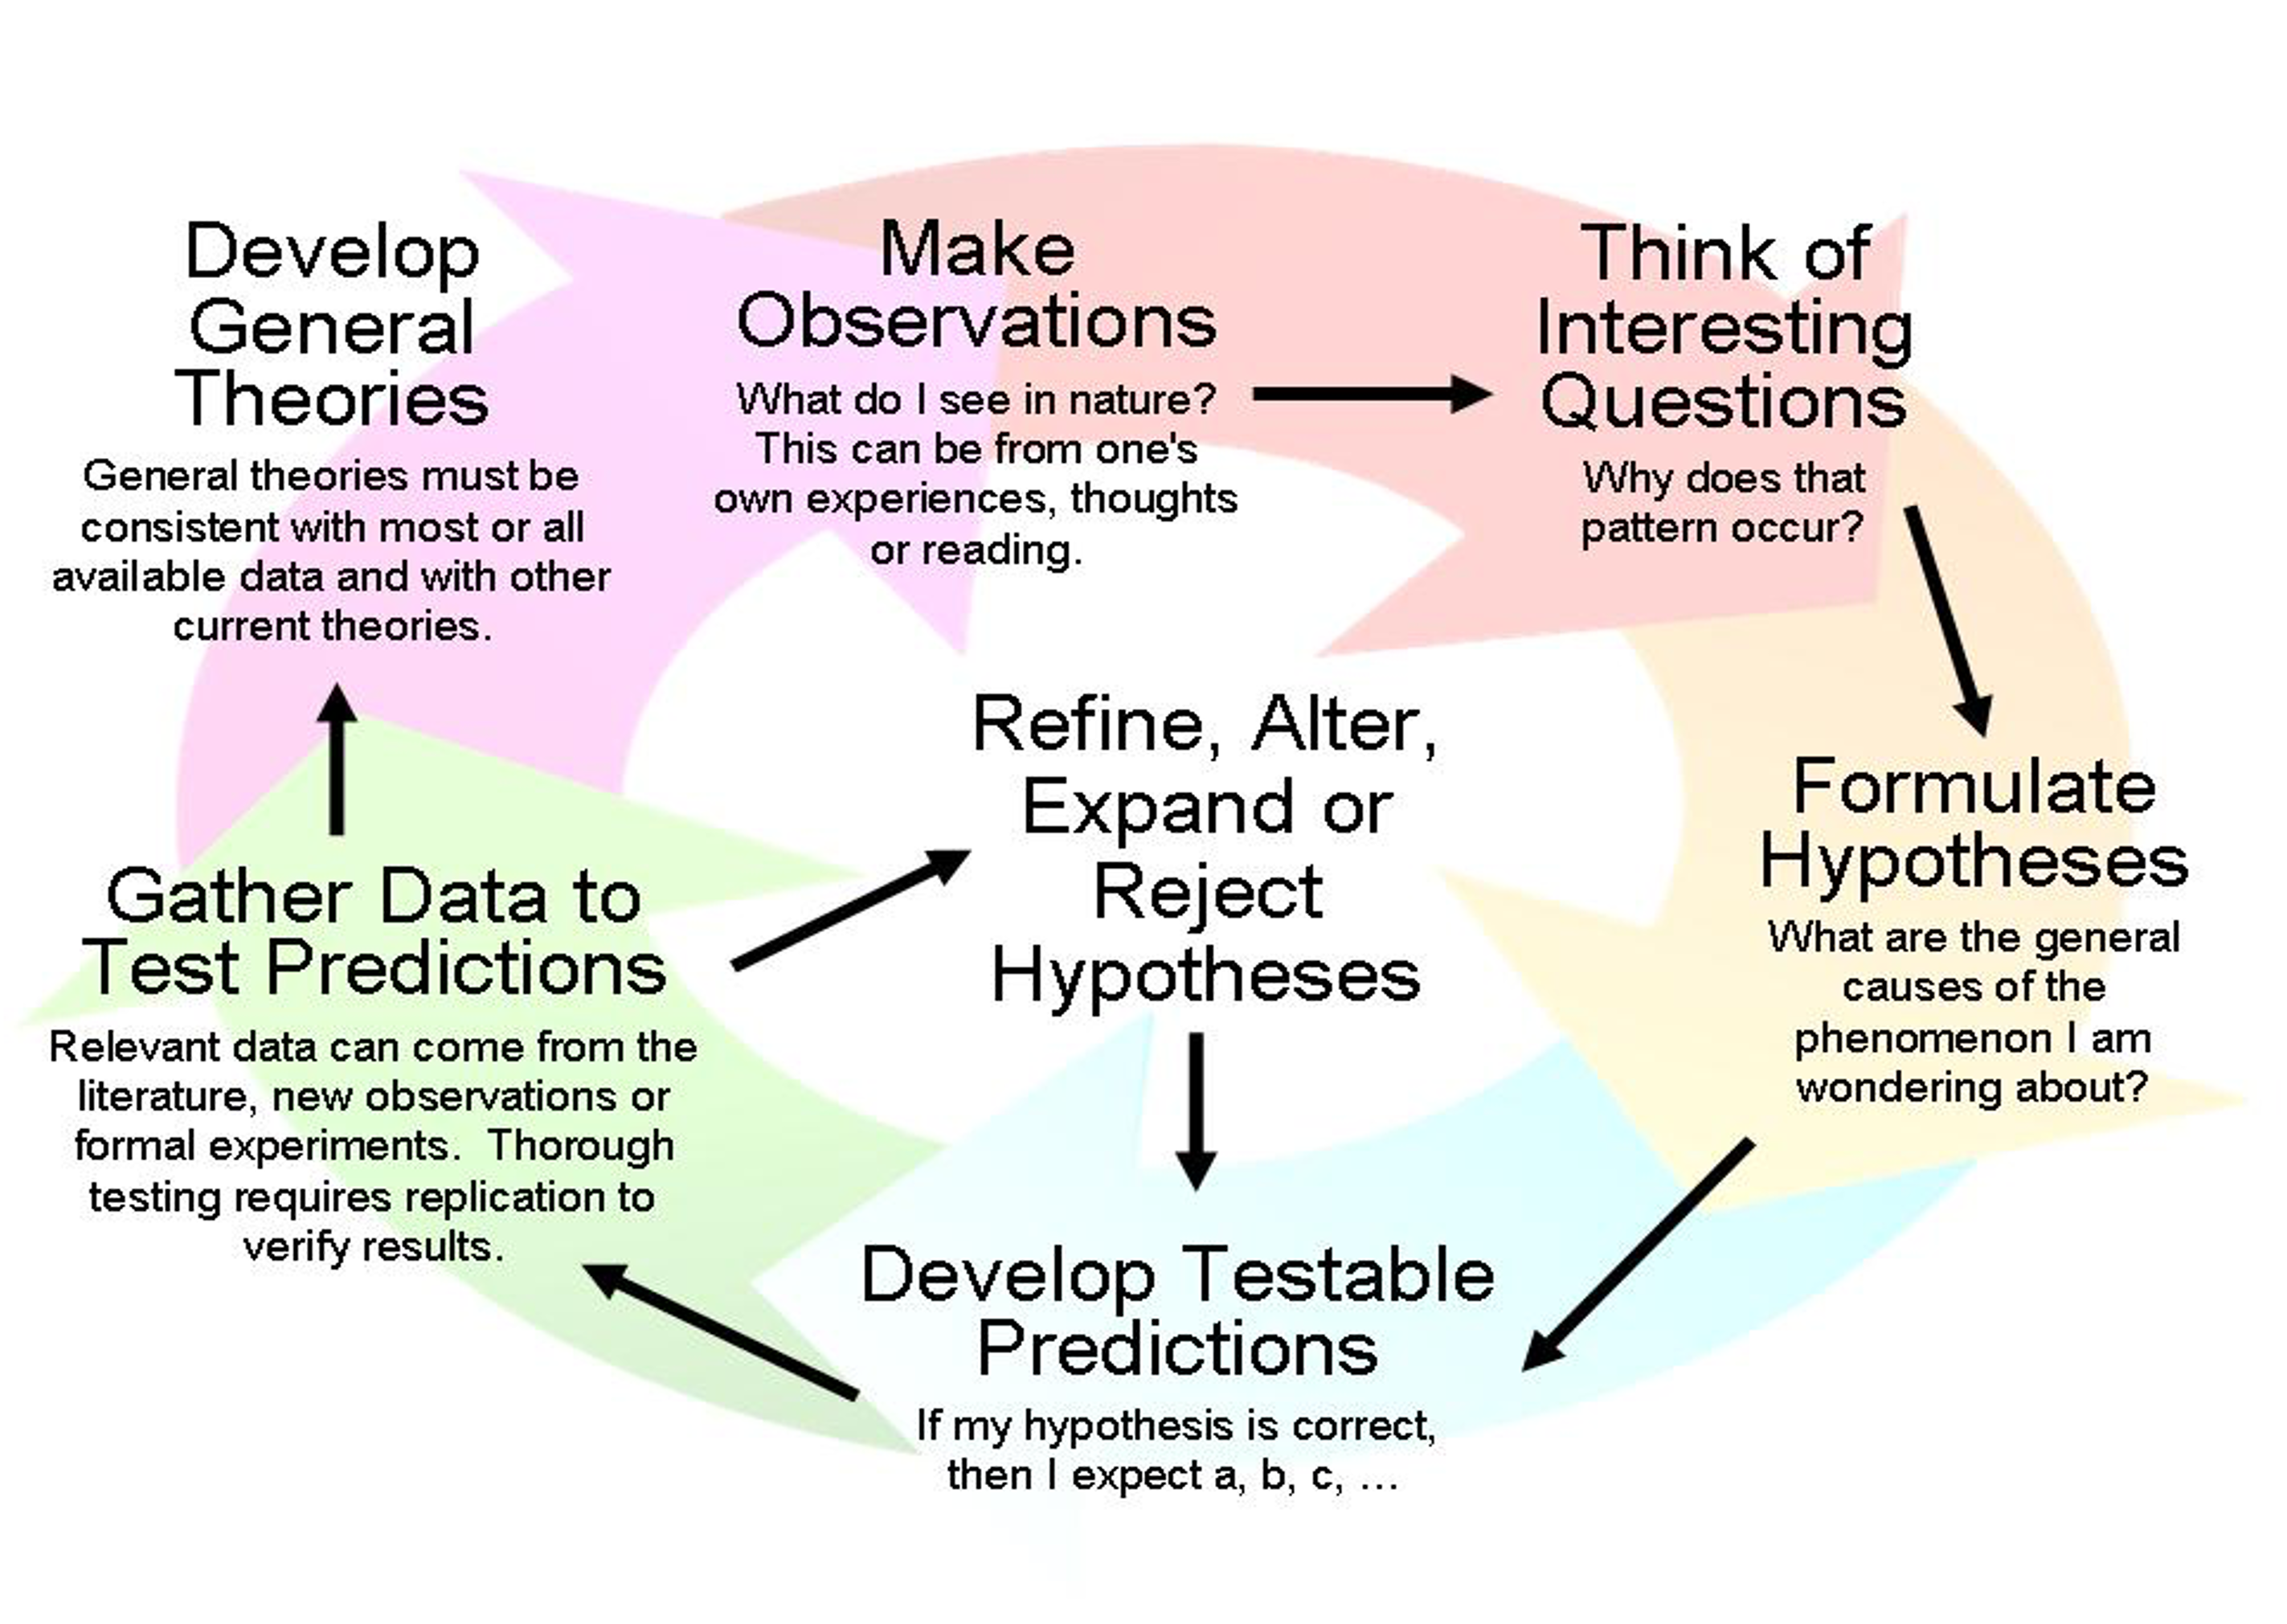
\includegraphics[width=39.53in]{/Users/craig.starbuck/Library/Mobile Documents/com~apple~CloudDocs/Documents/People Analytics Book/GitHub/peopleanalytics_lifecycle_book/graphics/Scientific Method} \caption{The Scientific Method}\label{fig:unnamed-chunk-2}
\end{figure}

Over the years, I have adapted the scientific method into a curtailed four-dimensional framework which is intended to elevate the rigor applied to the end-to-end analytical process. The four dimensions are (a) Discover, (b) Design, (c) Develop, and (d) Deliver, and this book will be organized around these. A checklist with general questions and considerations across the analytics lifecycle can be found in the Appendix.

\begin{figure}
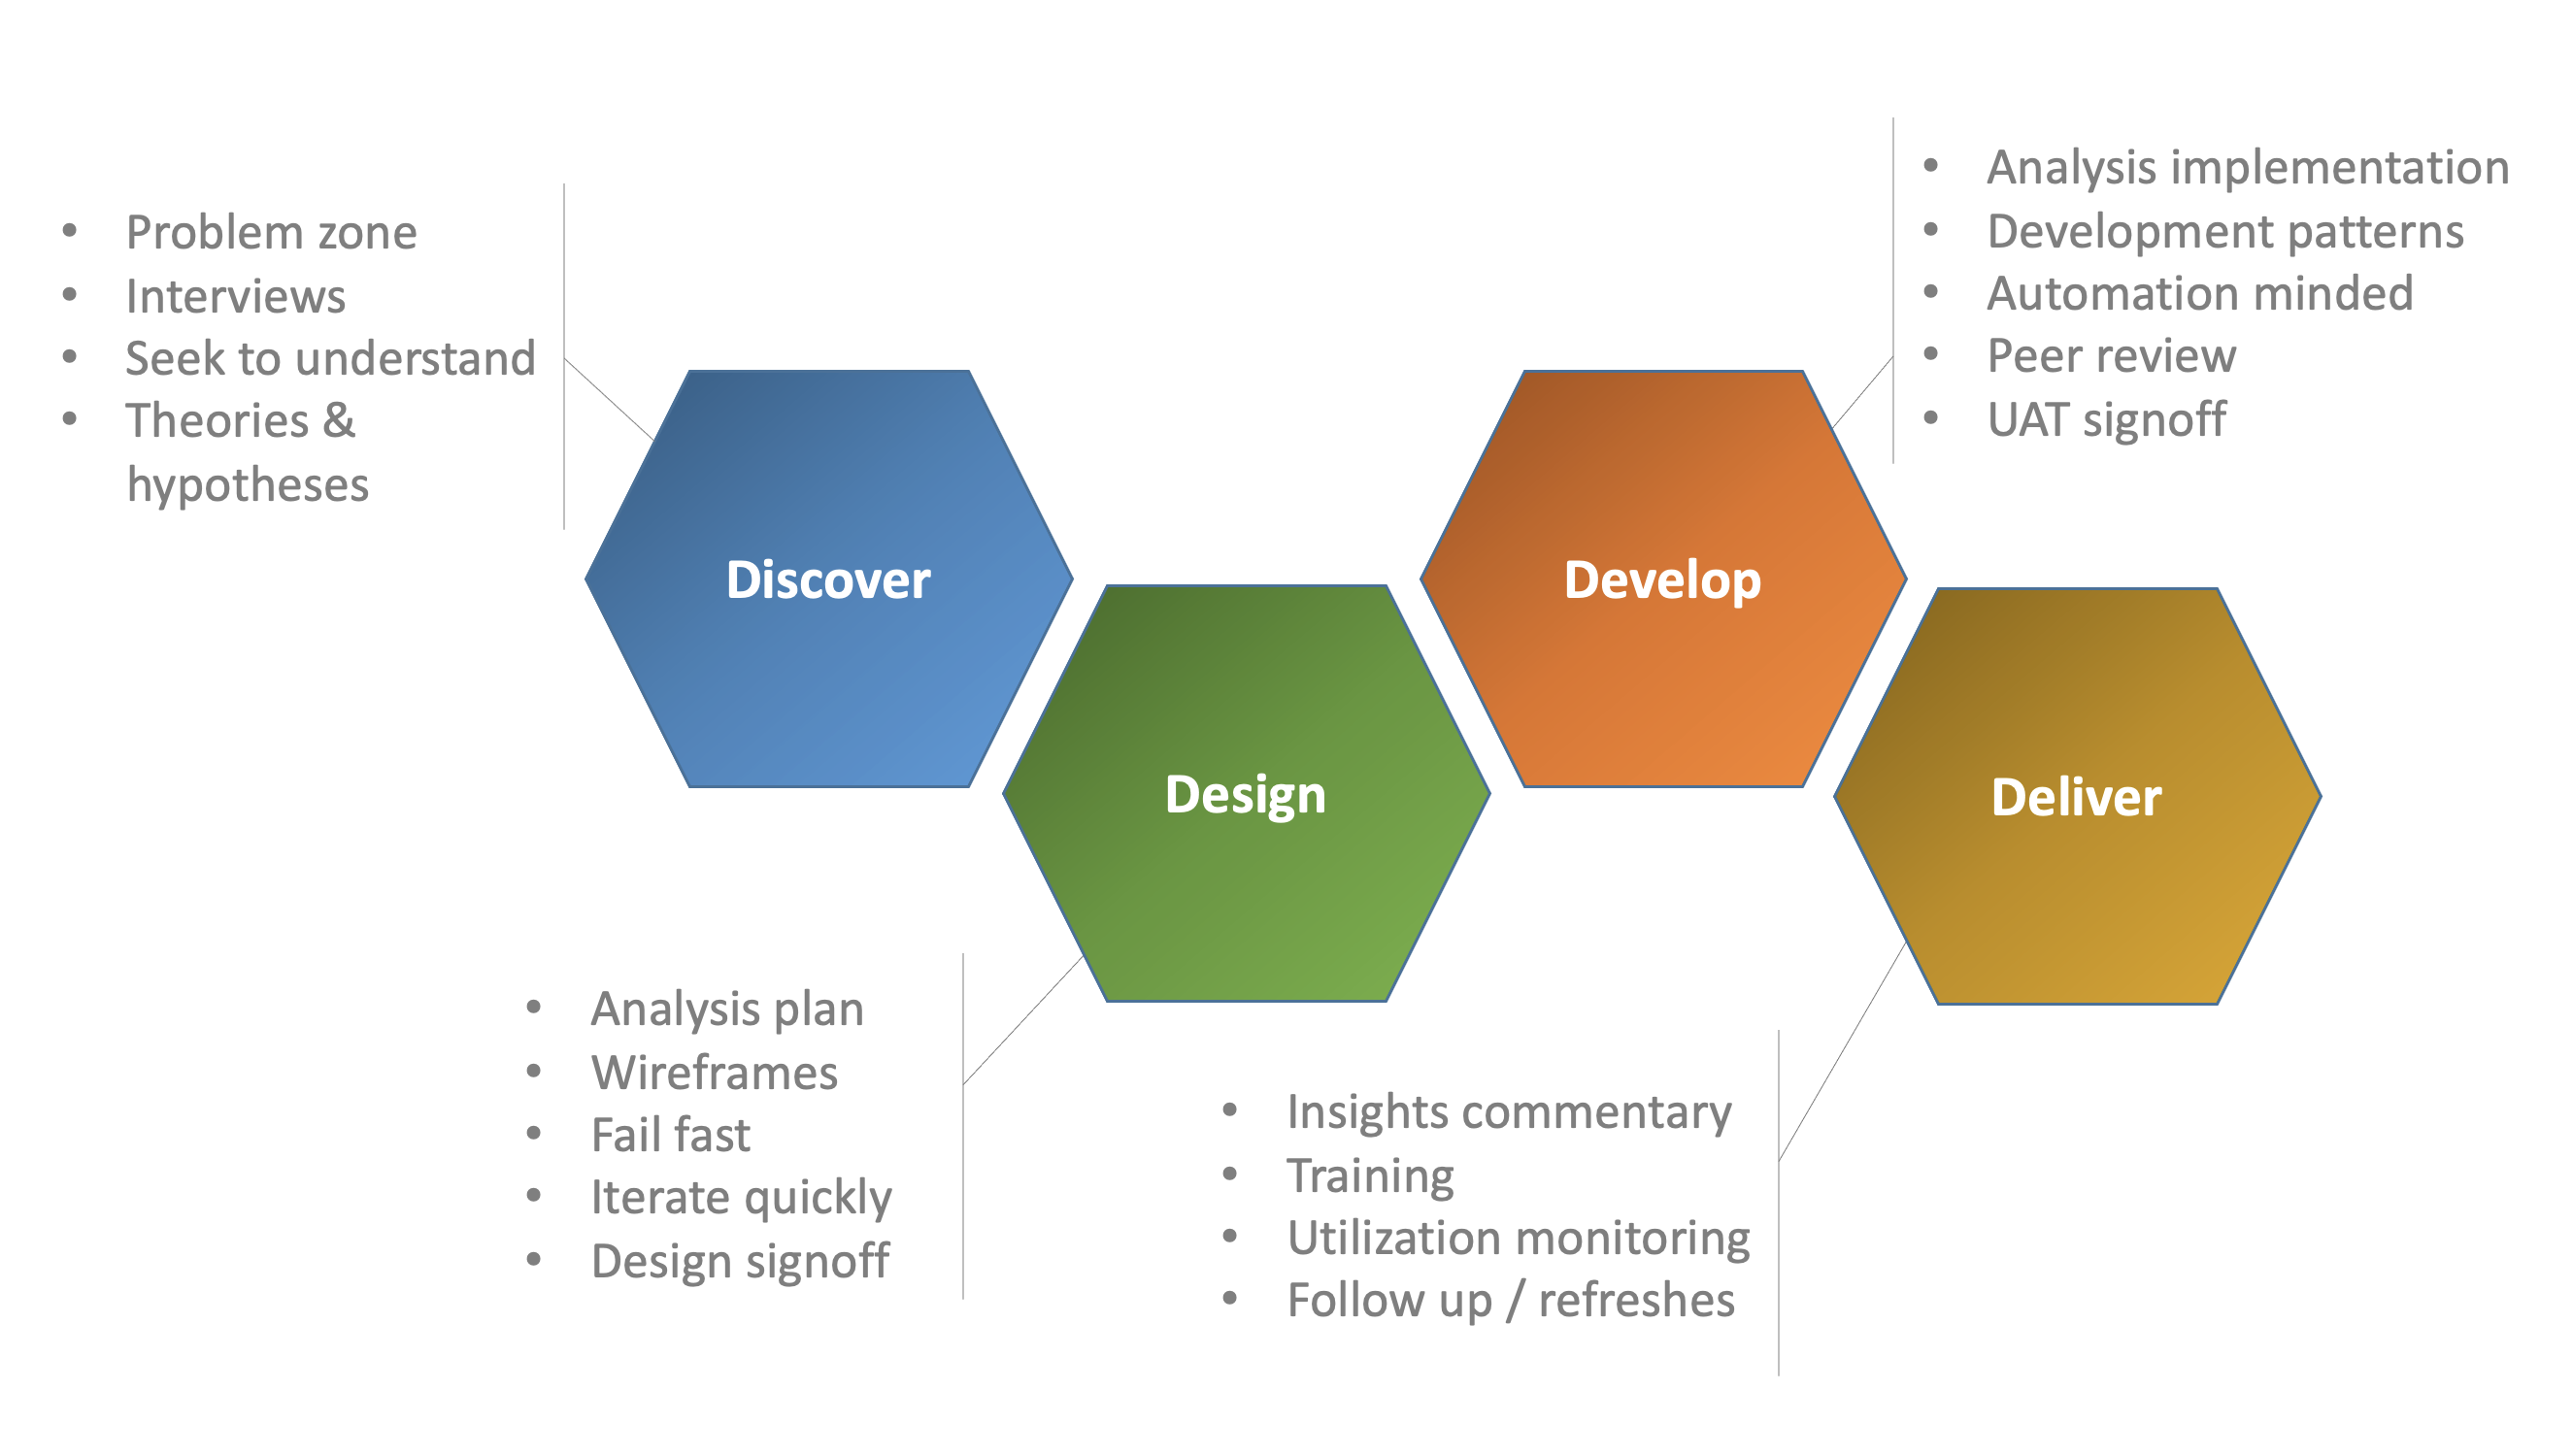
\includegraphics[width=36.81in]{/Users/craig.starbuck/Library/Mobile Documents/com~apple~CloudDocs/Documents/People Analytics Book/GitHub/peopleanalytics_lifecycle_book/graphics/4D Framework Overview} \caption{4D Framework}\label{fig:unnamed-chunk-3}
\end{figure}

1. Discover

You are likely familiar with the old adage: ``An ounce of prevention is worth a pound of cure.'' Such is the case with respect to planning in an analytics context. During the Discover phase, it is important to remain in the problem zone; seek to understand your clients' needs through active listening and questions. This is not the time for solutioning or committing to any specific deliverables. If the client's needs are ambiguous, proceeding will likely be an exercise in futility. Outlined below is a set of general questions that should be considered during this initial phase to prevent allocating scarce time and resourcing to a project that ultimately misses the mark.

2. Design

Perhaps the most important initial question to answer in the design phase is: ``Does anything already exist that addresses part, or all, of the client's objectives?'' If the existing solution will suffice, it's possible that there is simply a communication/education gap, and you can allocate time and resources elsewhere.

The end-user experience is of paramount importance during the Design phase, as solutions should have a consistent look and feel regardless of who developed the product. To achieve this, it is important to resist siloed thinking and consider the broader set of analytics solutions the team has delivered -- or is in the process of delivering.

3. Develop

4. Deliver

The Deliver phase can take many forms depending on the solution being released. If the solution is designed for a large user base, a series of recorded trainings may be in order so that there is a helpful reference for those unable to attend the live sessions or new joiners in the future. It is important to monitor success measures, which could be insights aligned to research hypotheses, dashboard utilization metrics, or any number of others defined within the Discover phase.

\hypertarget{research-methods}{%
\chapter{Research Methods}\label{research-methods}}

\hypertarget{statistical-fundamentals}{%
\chapter{Statistical Fundamentals}\label{statistical-fundamentals}}

\hypertarget{population-parameters}{%
\section{Population Parameters}\label{population-parameters}}

\hypertarget{sample-statistics}{%
\section{Sample Statistics}\label{sample-statistics}}

\hypertarget{descriptive-statistics}{%
\section{Descriptive Statistics}\label{descriptive-statistics}}

\begin{itemize}
\item
  Measures of Central Tendency

  Mean

  Perhaps the most intuitive measure of central tendency is the mean, which is often referred to as the average. The mean of a sample is denoted by \(\bar{x}\) and is defined by:

  \[ \bar{X} = \frac{\sum_{i=1}^{n} x_{i}}{n} \]
\end{itemize}

The mean of a set of numeric values can be calculated using the mean() function in R:

\begin{Shaded}
\begin{Highlighting}[]
\CommentTok{# Fill vector x with integers}
\NormalTok{x <-}\StringTok{ }\KeywordTok{c}\NormalTok{(}\DecValTok{1}\NormalTok{,}\DecValTok{1}\NormalTok{,}\DecValTok{1}\NormalTok{,}\DecValTok{2}\NormalTok{,}\DecValTok{2}\NormalTok{,}\DecValTok{2}\NormalTok{,}\DecValTok{3}\NormalTok{,}\DecValTok{3}\NormalTok{,}\DecValTok{4}\NormalTok{,}\DecValTok{50}\NormalTok{)}

\CommentTok{# Calculate average of vector x}
\KeywordTok{mean}\NormalTok{(x)}
\end{Highlighting}
\end{Shaded}

\begin{verbatim}
## [1] 6.9
\end{verbatim}

Median

The median represents the midpoint in a sorted vector of numbers. For vectors with an even number of values, the median is the average of the middle two numbers; it is simply the middle number for vectors with an odd number of values. When the distribution of data is skewed, or there is an extreme value like we observe in vector x, the median is a better measure of central tendency.

The median() function in R can be used to handle the sorting and midpoint selection:

\begin{Shaded}
\begin{Highlighting}[]
\CommentTok{# Calculate median of vector x}
\KeywordTok{median}\NormalTok{(x)}
\end{Highlighting}
\end{Shaded}

\begin{verbatim}
## [1] 2
\end{verbatim}

In this example, the median is only 2 compared with the mean of 6.9 (which is not really representative of any of the values in vector x). Large deltas between mean and median values are evidence of outliers.

Mode

The mode is the most frequent number in a set of values.

While mean() and median() are standard functions in R, mode() returns the internal storage mode of the object rather than the statistical mode of the data. We can easily create a function to return the statistical mode(s):

\begin{Shaded}
\begin{Highlighting}[]
\CommentTok{# Create function to calculate statistical mode(s)}
\NormalTok{stat.mode <-}\StringTok{ }\ControlFlowTok{function}\NormalTok{(x) \{}
\NormalTok{  ux <-}\StringTok{ }\KeywordTok{unique}\NormalTok{(x)}
\NormalTok{  tab <-}\StringTok{ }\KeywordTok{tabulate}\NormalTok{(}\KeywordTok{match}\NormalTok{(x, ux))}
\NormalTok{  ux[tab }\OperatorTok{==}\StringTok{ }\KeywordTok{max}\NormalTok{(tab)]}
\NormalTok{\}}

\CommentTok{# Return mode(s) of vector x}
\KeywordTok{stat.mode}\NormalTok{(x)}
\end{Highlighting}
\end{Shaded}

\begin{verbatim}
## [1] 1 2
\end{verbatim}

In this case, we have a bimodal distribution since both 1 and 2 occur most frequently.

Range

The range is the difference between the maximum and minimum values in a set of numbers.

The range() function in R returns the minimum and maximum numbers:

\begin{Shaded}
\begin{Highlighting}[]
\CommentTok{# Return lowest and highest values of vector x}
\KeywordTok{range}\NormalTok{(x)}
\end{Highlighting}
\end{Shaded}

\begin{verbatim}
## [1]  1 50
\end{verbatim}

We can leverage the max() and min() functions to calculate the difference between these values:

\begin{Shaded}
\begin{Highlighting}[]
\CommentTok{# Calculate range of vector x}
\KeywordTok{max}\NormalTok{(x, }\DataTypeTok{na.rm =} \OtherTok{TRUE}\NormalTok{) }\OperatorTok{-}\StringTok{ }\KeywordTok{min}\NormalTok{(x, }\DataTypeTok{na.rm =} \OtherTok{TRUE}\NormalTok{)}
\end{Highlighting}
\end{Shaded}

\begin{verbatim}
## [1] 49
\end{verbatim}

\begin{itemize}
\item
  Measures of Spread

  Variance

  Variance is a measure of the variability around the average value. Variance is calculated using the average of squared differences from the mean.

  Variance of a population is defined by:

  \[ \sigma^{2} = \frac{\sum (X_{i}-\mu)^{2}}{N} \]

  Variance of a sample is defined by:

  \[ s^{2} = \frac{\sum (x_{i}-\bar{x})^{2}}{n-1} \]

  It is important to note that since differences are squared, the variance is always non-negative. In addition, we cannot compare these squared differences to the arithmetic mean since the units are different. For example, if we calculate the variance of compensation measured in USD, variance should be expressed as USD squared while the mean exists in the original USD unit of measurement.

  Standard Deviation

  The standard deviation is simply the square root of the variance, as defined by:

  \[ s = \sqrt{\frac{\sum (x_{i} - \bar{x})^{2}}{N - 1}} \]

  Since a squared value can be converted back to its original units by taking its square root, the standard deviation expresses variability around the mean in the variable's original units.

  Quartiles

  The Interquartile Range (IQR)\ldots{}

  Covariance
\end{itemize}

\[ cov_{x,y} = \frac{\sum_{i=1}^{N}(x_{i}-\bar{x})(y_{i}-\bar{y})}{N-1} \]

Correlation

``Correlation is not causation.''

\[ r = frac{Nsum{XY}-(sum{X}sum{Y})}{sqrt{ [N sum{x^2}-(sum{x})^2][N sum{y^2}-(sum{y})^2 }]} \]

\hypertarget{inferential-statistics}{%
\section{Inferential Statistics}\label{inferential-statistics}}

The objective of inferential statistics is to make inferences -- with some degree of confidence -- about a population based on available sample data, and there are several concepts fundamental to this goal.

\begin{itemize}
\item
  Introduction to Probability
\item
  Central Limit Theorem
\end{itemize}

The Central Limit Theorem (CLT) is a mainstay of statistics and probability and fundamental to understanding the mechanics of inferential analysis techniques we will cover later in this book. The CLT was unpopular when initially coined by a French-born mathematician named Abraham De Moivre in the 1700s, but was later reintroduced and attracted new interest from theorists and academics (Daw \& Pearson, 1972).

The CLT states that the average of independent random variables, when increased in number, tend to follow a normal distribution. The distribution of sample means approaches a normal distribution regardless of the shape of the population distribution from which the samples are drawn. This is important because the normal distribution has properties that can be used to test the likelihood that an observed difference or relationship in a sample is also present in the population.

If we need to estimate the average value of a population, for example, we can lean on the CLT and normal distribution properties to obtain the range of values that are likely to include the true population average. This is how confidence intervals are defined, which enable us to make reasonable inferences about the unknown population parameters based on the sample data available from said population.

\begin{figure}
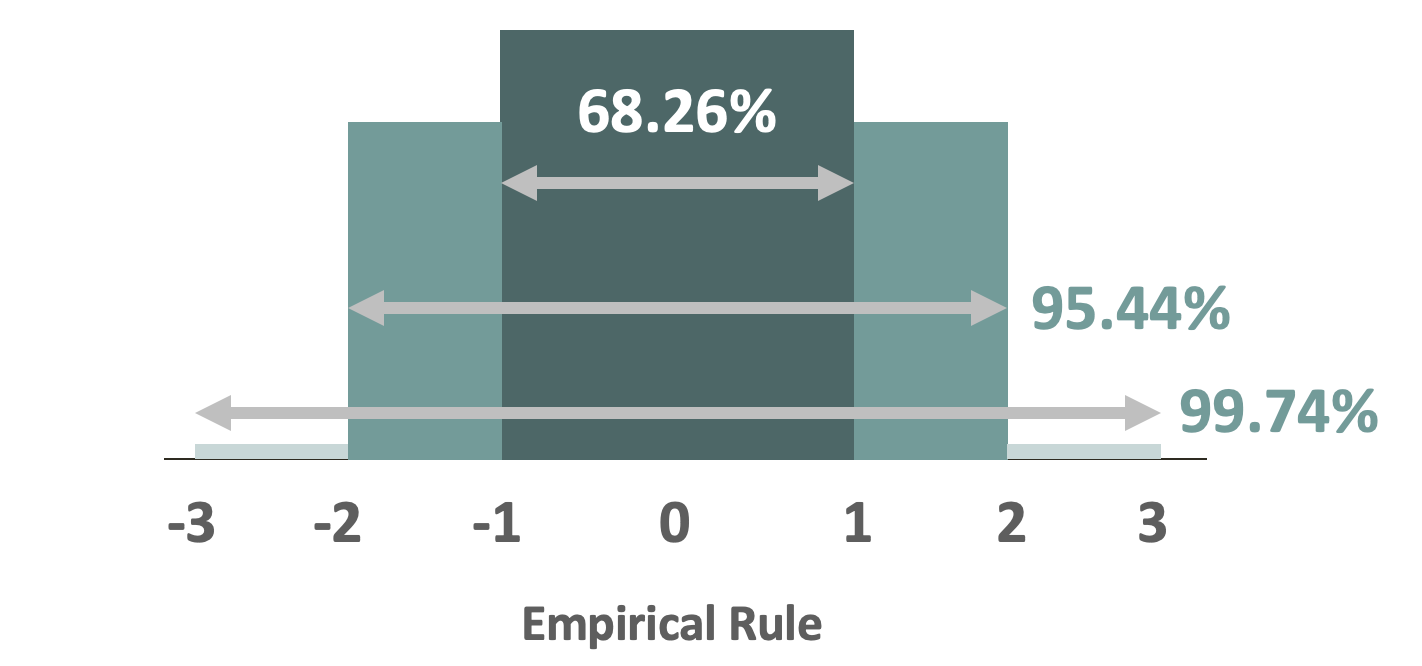
\includegraphics[width=19.75in]{/Users/craig.starbuck/Library/Mobile Documents/com~apple~CloudDocs/Documents/People Analytics Book/GitHub/peopleanalytics_lifecycle_book/graphics/Normal Distribution} \caption{Normal Distribution Properties}\label{fig:unnamed-chunk-9}
\end{figure}

Let's begin with an intuitive example of CLT, which has been inspired by Wheelan (2013). Consider a situation in which one of many buses shuttling 40 basketball players to a tournament finds itself lost. You receive word that a bus of lost people is discovered, and your job is to determine whether this bus is the missing bus of basketball players rather than some other bus of lost people. Consider also that a state fair is occurring the same day as the basketball tournament, and this event also has shuttles transporting groups of 40 people from their vehicles to the event.

Let's assume the mean and standard deviation of the height of these two groups are known; the group of basketball players are, on average, 6' 5'' with a standard deviation of 1'', while state fair attendees are, on average, a much shorter 5' 4'' with a wider standard deviation of 3''. With a known population mean and standard deviation, the standard error (standard deviation of the sample means) provides the ability to calculate the probability that the sample (the lost bus of people) belongs to the population of interest (basketball players competing in the tournament).

Herein lies the beauty of the CLT: roughly 68 percent of sample means will lie within one standard error of the population mean, roughly 95 percent will lie within two standard errors of the population mean, and roughly 99 percent will lie within three standard errors of the population mean. Therefore, any bus whose members have an average height that is not within two standard errors of the population mean (between 6' 3'' and 6' 7'' in the case of our basketball players) is statistically unlikely to be the bus of basketball players for which we are searching. This is because in less than 5 in 100 cases could we randomly draw a `reasonably sized' sample of basketball players with an average height so extremely different from the population average.

Because small samples lend to anamalies, we could -- by chance -- select a single person who happens to fall in the tails (very short or very tall relative to others); however, as the sample size increases, it becomes more and more likely that the observed average reflects the average of the larger population. It would be virtually impossible (in less than 1 in 100 times) to draw a random sample of players from the population with an average height that is not within three standard errors of the population mean (between 6' 2'' and 6' 8''). Therefore, if we find that the lost bus of people have an average height of 5' 11'', we should keep looking for our bus of basketball players.

Let's now see the CLT in action by simulating a random uniform population distribution from which we can draw random samples. Remember, the shape of the population distribution does not matter; we could simulate an Exponential, Gamma, Poisson, or other distribution and observe the same behavior.

\begin{Shaded}
\begin{Highlighting}[]
\CommentTok{# Load libraries for data wrangling and viz}
\KeywordTok{library}\NormalTok{(dplyr)}
\KeywordTok{library}\NormalTok{(ggplot2)}

\CommentTok{# Set seed for reproducible random distribution}
\KeywordTok{set.seed}\NormalTok{(}\DecValTok{1234}\NormalTok{)}

\CommentTok{# Generate uniform population distribution with 1000 values ranging from 1 to 100}
\NormalTok{rand.unif <-}\StringTok{ }\KeywordTok{runif}\NormalTok{(}\DecValTok{1000}\NormalTok{, }\DataTypeTok{min =} \DecValTok{1}\NormalTok{, }\DataTypeTok{max =} \DecValTok{100}\NormalTok{)}

\CommentTok{# Produce histogram to visualize population distribution}
\KeywordTok{ggplot}\NormalTok{() }\OperatorTok{+}\StringTok{ }
\StringTok{  }\KeywordTok{aes}\NormalTok{(rand.unif) }\OperatorTok{+}\StringTok{ }
\StringTok{  }\KeywordTok{labs}\NormalTok{(}\DataTypeTok{x =} \StringTok{"x"}\NormalTok{, }\DataTypeTok{y =} \StringTok{"N"}\NormalTok{) }\OperatorTok{+}\StringTok{ }
\StringTok{  }\KeywordTok{geom_histogram}\NormalTok{(}\DataTypeTok{colour =} \StringTok{"white"}\NormalTok{, }\DataTypeTok{size =} \FloatTok{.1}\NormalTok{, }\DataTypeTok{fill =} \StringTok{"#262626"}\NormalTok{)}
\end{Highlighting}
\end{Shaded}

\begin{figure}

{\centering 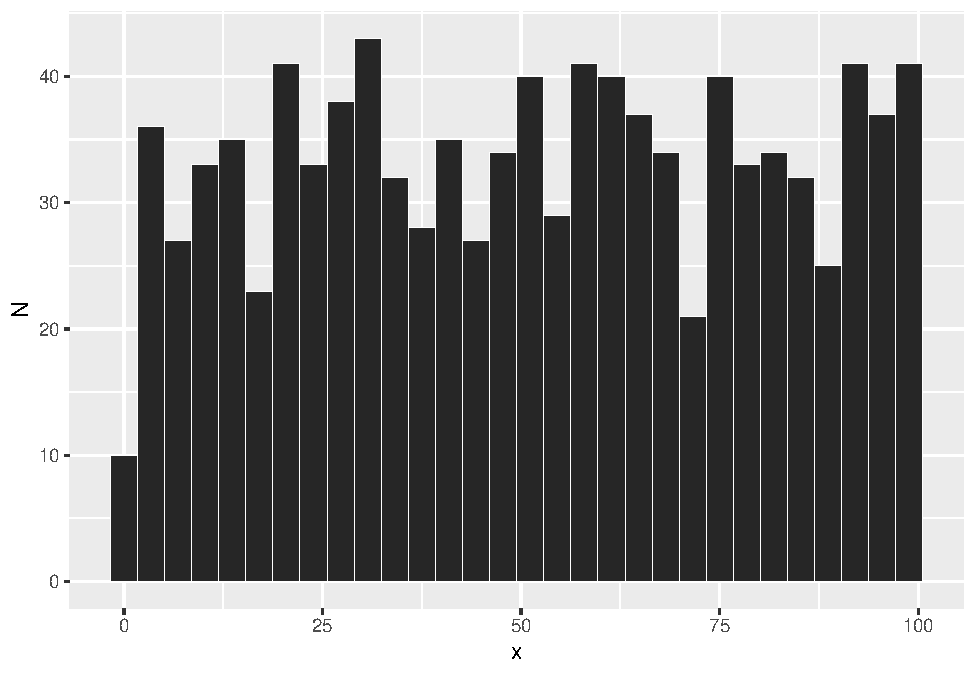
\includegraphics{_main_files/figure-latex/unnamed-chunk-10-1} 

}

\caption{Random Uniform Population Distribution (N = 1000)}\label{fig:unnamed-chunk-10}
\end{figure}

As expected, these randomly generated data are uniformly distributed. Next, we will draw 100 random samples of size 1 through 10 and plot the average of each.

\begin{Shaded}
\begin{Highlighting}[]
\CommentTok{# Define number of samples to draw from population distribution}
\NormalTok{samples <-}\StringTok{ }\DecValTok{100}

\CommentTok{# Populate vector with sample sizes}
\NormalTok{sample_n <-}\StringTok{ }\KeywordTok{c}\NormalTok{(}\DecValTok{1}\OperatorTok{:}\DecValTok{10}\NormalTok{)}

\CommentTok{# Initialize empty data frame to hold sample means}
\NormalTok{sample_means =}\StringTok{ }\OtherTok{NULL}

\CommentTok{# Set seed for reproducible random samples}
\KeywordTok{set.seed}\NormalTok{(}\DecValTok{456}\NormalTok{)}

\CommentTok{# For each n, draw random samples}
\ControlFlowTok{for}\NormalTok{ (n }\ControlFlowTok{in}\NormalTok{ sample_n) \{}
  
  \ControlFlowTok{for}\NormalTok{ (draw }\ControlFlowTok{in} \DecValTok{1}\OperatorTok{:}\NormalTok{samples) \{}
    
      \CommentTok{# Store sample means in data frame}
\NormalTok{      sample_means <-}\StringTok{ }\KeywordTok{rbind}\NormalTok{(sample_means, }\KeywordTok{cbind.data.frame}\NormalTok{(}
                            \DataTypeTok{n =}\NormalTok{ n, }
                            \DataTypeTok{x_bar =} \KeywordTok{mean}\NormalTok{(}\KeywordTok{sample}\NormalTok{(rand.unif, n, }\DataTypeTok{replace =} \OtherTok{TRUE}\NormalTok{, }\DataTypeTok{prob =} \OtherTok{NULL}\NormalTok{))))}
\NormalTok{  \}}
\NormalTok{\}}

\CommentTok{# Produce histograms to visualize distributions of sample means}
\NormalTok{sample_means }\OperatorTok\StringTok{ }\KeywordTok{ggplot}\NormalTok{() }\OperatorTok{+}\StringTok{ }
\StringTok{  }\KeywordTok{aes}\NormalTok{(}\DataTypeTok{x =}\NormalTok{ x_bar, }\DataTypeTok{fill =}\NormalTok{ n) }\OperatorTok{+}\StringTok{ }
\StringTok{  }\KeywordTok{labs}\NormalTok{(}\DataTypeTok{x =} \StringTok{"x-bar"}\NormalTok{, }\DataTypeTok{y =} \StringTok{"n"}\NormalTok{) }\OperatorTok{+}\StringTok{ }
\StringTok{  }\KeywordTok{geom_histogram}\NormalTok{(}\DataTypeTok{colour =} \StringTok{"white"}\NormalTok{, }\DataTypeTok{size =} \FloatTok{.1}\NormalTok{, }\DataTypeTok{fill =} \StringTok{"#262626"}\NormalTok{) }\OperatorTok{+}\StringTok{ }
\StringTok{  }\KeywordTok{facet_wrap}\NormalTok{(}\OperatorTok{~}\NormalTok{n)}
\end{Highlighting}
\end{Shaded}

\begin{figure}

{\centering 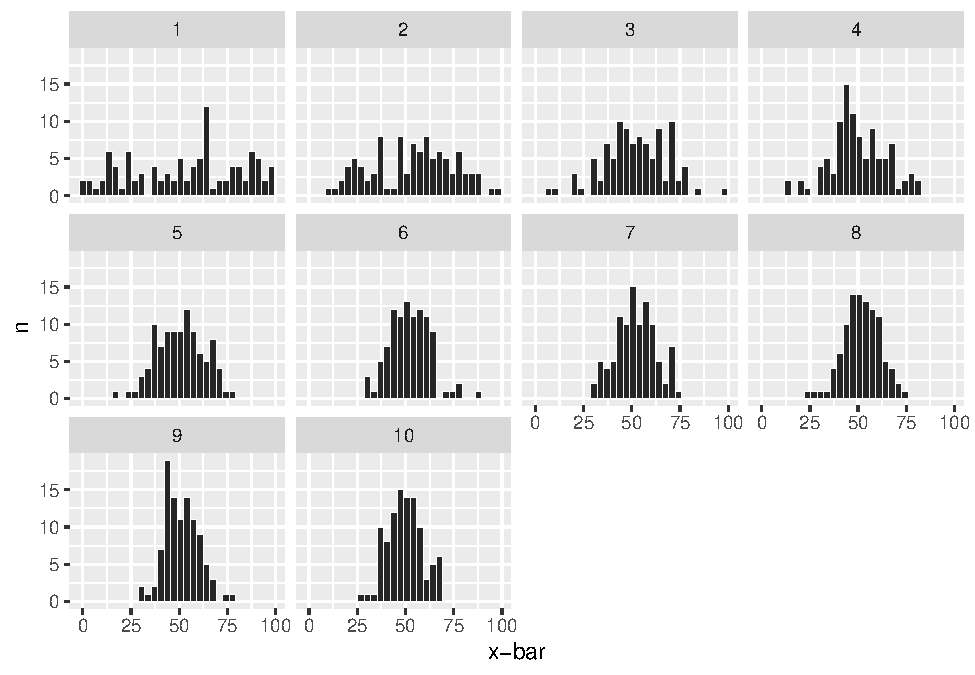
\includegraphics{_main_files/figure-latex/unnamed-chunk-11-1} 

}

\caption{Distribution of 100 Sample Means (n = 1-10)}\label{fig:unnamed-chunk-11}
\end{figure}

Per the CLT, we can see that as n increases, the sample means become more normally distributed.

\begin{itemize}
\item
  Confidence Intervals

  A Confidence Interval (CI) is a range of values that likely includes an unknown population value. A related concept that is fundamental to estimating CIs is the standard error. The standard error (SE) is the standard deviation of sample means. While the standard deviation is a measure of variability for random variables, the variability captured by the SE reflects how representative the sample is of the population. Since sample statistics will approach the actual population parameters as the size of the sample increases, the SE and sample size are inversely related; that is, the SE decreases as the sample size increases. The SE is defined by:

  \[ SE = \frac{\sigma}{\sqrt{n}} \]

  Let's illustrate the relationship between CIs and standard errors by validating whether the normal distribution properties are characteristic of the data simulated for our CLT example:
\end{itemize}

\begin{Shaded}
\begin{Highlighting}[]
\CommentTok{# Store sample means with n = 10}
\NormalTok{x_bars <-}\StringTok{ }\NormalTok{sample_means[sample_means}\OperatorTok{$}\NormalTok{n }\OperatorTok{==}\StringTok{ }\DecValTok{10}\NormalTok{, }\StringTok{"x_bar"}\NormalTok{]}

\CommentTok{# Calculate 95% CI (1.96 standard errors above and below the mean)}
\NormalTok{ci95_upper_bound <-}\StringTok{ }\KeywordTok{mean}\NormalTok{(x_bars) }\OperatorTok{+}\StringTok{ }\KeywordTok{sd}\NormalTok{(x_bars) }\OperatorTok{*}\StringTok{ }\FloatTok{1.96}
\NormalTok{ci95_lower_bound <-}\StringTok{ }\KeywordTok{mean}\NormalTok{(x_bars) }\OperatorTok{-}\StringTok{ }\KeywordTok{sd}\NormalTok{(x_bars) }\OperatorTok{*}\StringTok{ }\FloatTok{1.96}

\CommentTok{# Calculate percent of sample means within 95% CI}
\KeywordTok{length}\NormalTok{(x_bars[x_bars }\OperatorTok{>}\StringTok{ }\NormalTok{ci95_lower_bound }\OperatorTok{&}\StringTok{ }\NormalTok{x_bars }\OperatorTok{<}\StringTok{ }\NormalTok{ci95_upper_bound]) }\OperatorTok{/}\StringTok{ }\KeywordTok{length}\NormalTok{(x_bars) }\OperatorTok{*}\StringTok{ }\DecValTok{100}
\end{Highlighting}
\end{Shaded}

\begin{verbatim}
## [1] 95
\end{verbatim}

As expected, 95\% of sample means are within our 95\% CI (+/- 1.96 standard errors). 1.96 is a z-score, which is simply the number of standard deviations (or SEs in this case) that correspond to the 95\% CI.

Next, let's look at a 99\% CI. We will use a z-score of 2.58 for this:

\begin{Shaded}
\begin{Highlighting}[]
\CommentTok{# Calculate 99% CI (2.58 standard errors above and below the mean)}
\NormalTok{ci99_upper_bound <-}\StringTok{ }\KeywordTok{mean}\NormalTok{(x_bars) }\OperatorTok{+}\StringTok{ }\KeywordTok{sd}\NormalTok{(x_bars) }\OperatorTok{*}\StringTok{ }\FloatTok{2.58}
\NormalTok{ci99_lower_bound <-}\StringTok{ }\KeywordTok{mean}\NormalTok{(x_bars) }\OperatorTok{-}\StringTok{ }\KeywordTok{sd}\NormalTok{(x_bars) }\OperatorTok{*}\StringTok{ }\FloatTok{2.58}

\CommentTok{# Calculate percent of sample means within 99% CI}
\KeywordTok{length}\NormalTok{(x_bars[x_bars }\OperatorTok{>}\StringTok{ }\NormalTok{ci99_lower_bound }\OperatorTok{&}\StringTok{ }\NormalTok{x_bars }\OperatorTok{<}\StringTok{ }\NormalTok{ci99_upper_bound]) }\OperatorTok{/}\StringTok{ }\KeywordTok{length}\NormalTok{(x_bars) }\OperatorTok{*}\StringTok{ }\DecValTok{100}
\end{Highlighting}
\end{Shaded}

\begin{verbatim}
## [1] 100
\end{verbatim}

All of the sample means are within the 99\% CI (+/- 2.58 standard errors), indicating that it would be highly unlikely -- nearly impossible even -- to observe a sample mean \texttt{from\ the\ same\ population} that falls outside this interval.

\hypertarget{measurement-sampling}{%
\chapter{Measurement \& Sampling}\label{measurement-sampling}}

\hypertarget{data-preparation}{%
\chapter{Data Preparation}\label{data-preparation}}

\hypertarget{data-wrangling}{%
\section{Data Wrangling}\label{data-wrangling}}

\hypertarget{feature-engineering}{%
\section{Feature Engineering}\label{feature-engineering}}

Level one people analytics tends to utilize only the delivered fields from the HRIS (e.g., location, job profile, org tenure, etc.), but a good next step is to derive smarter variables from these fields. These can then be used to slice and dice turnover and engagement data differently, use as inputs in attrition risk models, etc. Below are some ideas to get you started:

\begin{itemize}
\tightlist
\item
  Number of jobs per unit of tenure (larger proportions tend to see greater career pathing)
\item
  Office/remote worker (binary variable dummy coded as 1/0)
\item
  Local/remote manager (binary variable dummy coded as 1/0)
\item
  Hire/Rehire (binary variable dummy coded as 1/0)
\item
  Hired/acquired (proxy for culture shock effects)
\item
  Gender isolation (ratio of employee's gender to number of the same within immediate work
  group)
\item
  Generation isolation (comparison of age bracket to most frequent generational bracket within
  immediate work group)
\item
  Ethnic isolation (ratio of employee's ethnicity to number of the same within immediate work
  group)
\item
  Difference between employee and manager age
\item
  Percentage change between last two performance appraisal scores (per competency and/or
  overall)
\item
  Team and department quit outbreak indicators (ratio of terms over x months relative to average
  headcount over x months)
\item
  Industry experience (binary or length in years)
\end{itemize}

Remember to compute variables consistent with a need (e.g., is there reason to believe generationally isolated employees are more likely to term?). There may be a time and place for undertaking data mining initiatives with no a priori theories about what may be uncovered; however, more often than not, our efforts should be tied to specific hypotheses the business needs tested, which have sound theoretical underpinnings.

\hypertarget{analysis-of-differences}{%
\chapter{Analysis of Differences}\label{analysis-of-differences}}

\hypertarget{comparing-2-distributions}{%
\section{Comparing 2 Distributions}\label{comparing-2-distributions}}

\hypertarget{comparing-3-distributions}{%
\section{Comparing 3+ Distributions}\label{comparing-3-distributions}}

\hypertarget{inferential-models}{%
\chapter{Inferential Models}\label{inferential-models}}

It's important to draw a distinction between inferential and predictive models. Inferential models are highly interpretable and their utility is largely in understanding the nature and magnitude of the effect variables have on outcomes. Inferential models also lend to quantifying the extent to which we can generalize the observed effects to the larger population from which the sample was drawn. The objective in predictive modeling is to also to learn from patterns in historical data but for the purpose of achieving the most accurate predictions of future events -- even at the expense of interpretability. To be clear, this isn't to say that predictive models cannot be interpreted -- they certainly can -- but I've seen relatively few applications for predictive modeling in people analytics because models generally need to be highly interpretable to support action planning.

This chapter is dedicated to inferential models to support a working understanding of how to interpret model output and communicate clear, data-driven narratives that respect the nuance and noise characteristic of people data. The following chapter will provide an overview of predictive modeling frameworks.

\hypertarget{regression}{%
\section{Regression}\label{regression}}

Regression is perhaps the most important statistical learning technique for people analytics. If you have taken a statistics course at the undergraduate or graduate levels, you have surely already encountered it. Before diving into the math to understand the mechanics of regression, let's develop an intuitive understanding.

Imagine we are sitting at a large public park in NYC on a nice fall afternoon. If asked to estimate the annual compensation of the next person to walk by, in the absence of any additional information how would you estimate this? Most would likely estimate the average annual compensation of everyone capable of walking by. Since this would include both residents and visitors, this would be a very large group of people! The obvious limitation with this approach is that among the large group of people capable of walking by, there is likely a significant range of annual compensation values. Many walking by may be children, unemployed, or retirees who earn no annual compensation, while others may be highly compensated senior executives at the pinnacle of their careers. Since the range of annual compensation could be zero to billions of dollars, estimating the average of such a large population is likely going to be highly inaccurate without more information about who may walk by.

Let's consider that we are sitting outside on a weekday afternoon. Should this influence our annual compensation estimate? It is likely that we can eliminate a large segment of those likely to walk by, as we would expect most children to be in school on a typical fall weekday afternoon. It's also unlikely that those who are employed and not on vacation will walk by on a fall weekday afternoon. Therefore, factoring in that it is a weekday should limit the size of the population which in turn may reduce the range of annual compensation values for our population of passerbys.

Let's now consider that the park is open only to invited guests for a symposium on people analytics. Though it may be difficult to believe, a relatively small subset of the population is likely interested in attending such a symposium, so this information will likely be very helpful in reducing the size of the population who could walk by, which should further reduce the range of annual compensation since we probably have a good idea of the profile of those most likely to attend. This probably also lessens (or altogether eliminates) the importance of the weekday factor in explaining why people vary in the amount of compensation they earn each year.

Furthermore, let's consider that only those who reside in NYC and Boise were invited, and that the next person to walk by resides in Boise. Most companies apply a significant cost of living multiplier to the compensation for those in an expensive region such as NYC, resulting in a significant difference in compensation relative to those residing in a much less expensive city like Boise -- all else being equal. Therefore, if we can partition attendees into two groups based on their geography, this should limit the range of annual compensation significantly within each -- likely making the average compensation amount in each group a more nuanced and reasonable estimate.

What if we also learn the specific zip code in which the next passerby from Boise resides? The important information is likely captured in the larger city label (NYC vs.~Boise), and the compensation for the specific zip codes within each city are unlikely to vary to a significant degree. Assuming this is true, it probably would not make sense to consider both the city name and zip code since they are effectively redundant pieces of information with regard to explaining differences in annual compensation.

What if we learn that the next person to walk by will be wearing a blue shirt? Does this influence your estimate? Unless there is research to suggest shirt color and earnings are related, this information will likely not contribute any significant information to our understanding of why people vary in the amount of compensation they earn annually and should, therefore, not be considered.

You can probably think of many relevant variables that would help further narrow the range of annual compensation. These may include job, level, years of experience, education, location, among other factors. The main thing to understand is that for each group of observations with the same characteristics -- such as senior analysts with a graduate degree who reside in NYC -- there is a distribution of annual compensation. This distribution reflects unexplained variance. That is, we do not have information to explain why the compensation for each and every person is not the same and in social science contexts, it simply is not practical to explain 100 percent of the variance in outcomes. Two people may be similar on hundreds of factors (experience, education, skills) but one was simply a more effective negotiator when offered the same role and commanded a higher salary. It's likely we do not have data on salary negotiation ability so this information would leave us with unexplained variance in compensation. The goal is simply to identify the variables that provide the most information in helping us tighten the distribution so that estimating the average value will generally be an accurate estimate for those in the larger population with the same characteristics.

While we can generally improve our estimates with more relevant information (not shirt color or residential zip code in this case), it is important to understand that samples which are too small (n \textless{} 30) lend to anomalies; modeling noise in sparse data can result in models that are unlikely to generalize beyond the sample data. For example, if the only people from Boise to attend the people analytics symposium happen to be two ultra wealthy tech entrepreneurs who earn millions each year, it would not be appropriate to use this as the basis for our estimates of all future attendees from Boise. This is a phenomenon known as overfitting that will be covered later in this chapter.

This is the essence of regression modeling: find a limited number of variables which independently or jointly provide significant information that helps explain (by reducing) variance around the average value. As illustrated in this example, adding additional variables (information) can impact the importance of other variables or may offer no incremental information at all. In the subsequent sections, we will cover how to identify which variables are important and how to quantify the effect they have on the outcome.

\hypertarget{simple-linear-regression}{%
\section{Simple Linear Regression}\label{simple-linear-regression}}

\hypertarget{parameter-estimation}{%
\subsection{Parameter Estimation}\label{parameter-estimation}}

Ordinary Least Squares (OLS) is the most common method for estimating unknown parameters in a linear regression model.

\hypertarget{multiple-linear-regression}{%
\section{Multiple Linear Regression}\label{multiple-linear-regression}}

\hypertarget{moderation}{%
\subsection{Moderation}\label{moderation}}

\hypertarget{mediation}{%
\subsection{Mediation}\label{mediation}}

\hypertarget{polynomial-regression}{%
\section{Polynomial Regression}\label{polynomial-regression}}

\hypertarget{logistic-regression}{%
\section{Logistic Regression}\label{logistic-regression}}

Logistic regression is an excellent tool when the outcome is categorical. Logistic regression allows us to model the probability of different classes -- a type of modeling often referred to as classification. The context for classification can be binomial for two classes (e.g., active/inactive, promoted/not promoted), multinomial for multiple unordered classes (e.g., skills, job families), or ordinal for multiple ordered classes (e.g., survey items measured on a Likert scale, performance level).

\hypertarget{binomial}{%
\subsection{Binomial}\label{binomial}}

\hypertarget{multinomial}{%
\subsection{Multinomial}\label{multinomial}}

\hypertarget{ordinal}{%
\subsection{Ordinal}\label{ordinal}}

Proportional Odds Logistic Regression

\hypertarget{hierarchical-models}{%
\section{Hierarchical Models}\label{hierarchical-models}}

\hypertarget{predictive-models}{%
\chapter{Predictive Models}\label{predictive-models}}

\hypertarget{bias-variance-trade-off}{%
\section{Bias-Variance Trade-Off}\label{bias-variance-trade-off}}

\hypertarget{cross-validation}{%
\section{Cross-Validation}\label{cross-validation}}

\hypertarget{balancing-classes}{%
\section{Balancing Classes}\label{balancing-classes}}

\hypertarget{model-performance}{%
\section{Model Performance}\label{model-performance}}

\hypertarget{automated-machine-learning-automl}{%
\chapter{Automated Machine Learning (AutoML)}\label{automated-machine-learning-automl}}

\hypertarget{unsupervised-learning-models}{%
\chapter{Unsupervised Learning Models}\label{unsupervised-learning-models}}

\hypertarget{factor-analysis}{%
\section{Factor Analysis}\label{factor-analysis}}

\hypertarget{clustering}{%
\section{Clustering}\label{clustering}}

\hypertarget{data-visualization}{%
\chapter{Data Visualization}\label{data-visualization}}

\hypertarget{data-storytelling}{%
\chapter{Data Storytelling}\label{data-storytelling}}

\hypertarget{bibliography}{%
\chapter{Bibliography}\label{bibliography}}

Baron, R. M., \& Kenny, D. A. (1986). The moderator--mediator variable distinction in social psychological research: Conceptual, strategic, and statistical considerations. Journal of Personality and Social Psychology, 51(6), 1173--1182.

Daw, R. H., \& Pearson, E. S. (1972). Studies in the History of Probability and Statistics. XXX. Abraham De Moivre's 1733 Derivation of the Normal Curve: A Bibliographical Note. Biometrika, 59(3), 677--680. \url{https://doi.org/10.2307/2334818}

James, G., Witten, D., Hastie, T., \& Tibshirani, R. (2013). An Introduction to Statistical Learning: With Applications in R. New York: Springer.

Kahneman, D. (2011). Thinking, fast and slow. New York: Farrar, Straus and Giroux.

Kerlinger, F., \& Lee, H. (2000). Foundations of behavioral research (4th ed.). Melbourne: Wadsworth.

Wheelan, C. (2013). Naked Statistics: Stripping the Dread from the Data. New York: W.W. Norton.

\hypertarget{appendix}{%
\chapter{Appendix}\label{appendix}}

\hypertarget{d-framework-1}{%
\section{4D Framework}\label{d-framework-1}}

\begin{figure}
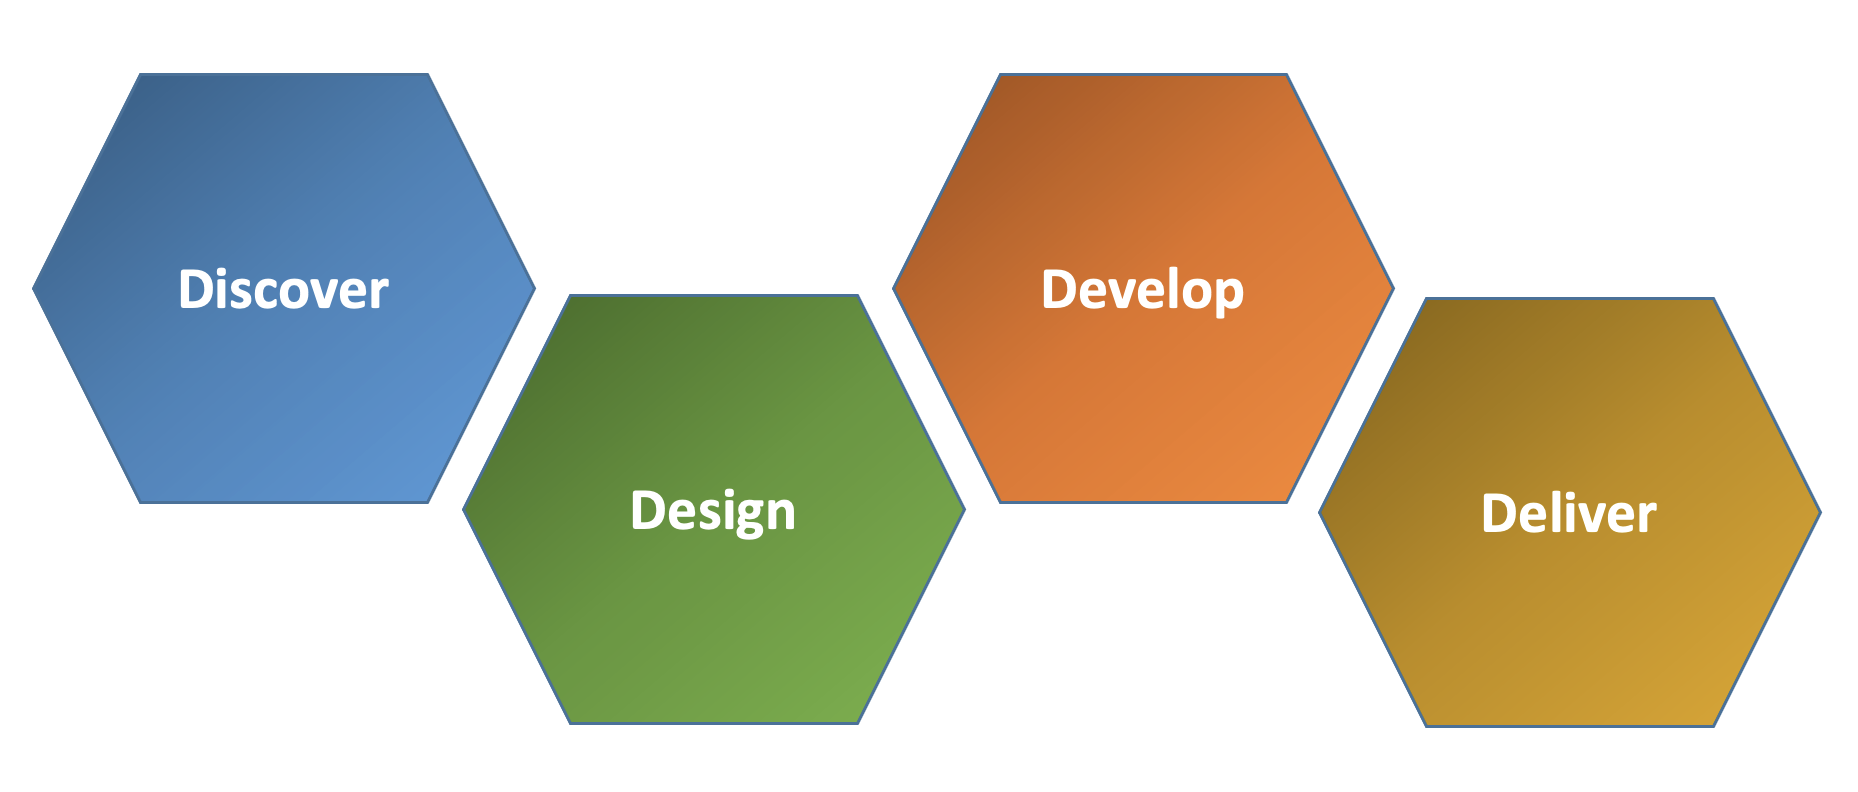
\includegraphics[width=25.81in]{/Users/craig.starbuck/Library/Mobile Documents/com~apple~CloudDocs/Documents/People Analytics Book/GitHub/peopleanalytics_lifecycle_book/graphics/4D Framework} \caption{Figure 1: 4D Framework}\label{fig:unnamed-chunk-14}
\end{figure}

1. Discover

You are likely familiar with the old adage: ``An ounce of prevention is worth a pound of cure.'' Such is the case with respect to planning in an analytics context. During the Discover phase, it is important to remain in the problem zone; seek to understand your clients' needs through active listening and questions. This is not the time for solutioning or committing to any specific deliverables. If the client's needs are ambiguous, proceeding will likely be an exercise in futility. Outlined below is a set of general questions that should be considered during this initial phase to prevent allocating scarce time and resourcing to a project that ultimately misses the mark.

\begin{itemize}
\item
  Client

  Who is the client? A client can be a person or organization that has contracting you for consulting services, or an internal stakeholder within your organization who has need. What is important to them?
\item
  Primary Objective

  \begin{itemize}
  \tightlist
  \item
    What is the client ultimately hoping to accomplish?
  \item
    Is the request merely to satisfy one's curiosity, or are there actions that can realistically be taken to materially influence said objective?
  \end{itemize}
\item
  Problem Statement

  \begin{itemize}
  \tightlist
  \item
    One of my most important early steps is clearly defining the problem statement. If your understanding of the problem -- after translating from the business terms in which it was initially expressed -- is misaligned with the client's needs, none of the subsequent steps matter.
  \end{itemize}
\item
  Guiding Theories

  \begin{itemize}
  \tightlist
  \item
    What theoretical explanations can the client offer as potential rationalizations for the phenomena of interest?
  \item
    Are there existing theories in the organizational literature that should guide how the problem is tackled (e.g., findings from similar research implemented in other contexts)?
  \end{itemize}
\item
  Research Questions

  To respect the nuances of the problem statement, it is important to unpack it and frame as a set of overarching questions to guide the research.

  \begin{itemize}
  \tightlist
  \item
    Q1: \ldots{}
  \item
    Q2: \ldots{}
  \item
    Q3: \ldots{}
  \end{itemize}
\item
  Research Hypotheses

  Once research questions are developed, what do you expect to find based on anecdotal stories or empirical findings? As a next step, these expectations should be expressed in the form of research hypotheses. Please note that these research hypotheses are different from statistical hypotheses.

  \begin{itemize}
  \tightlist
  \item
    H1: \ldots{}
  \item
    H2: \ldots{}
  \item
    H3: \ldots{}
  \end{itemize}

  To ensure the hypotheses lend themselves to actionable analyses, it is important to consider the following: ``What does success look like?'' In other words, once the project is complete, against which success measures will the project's success be determined? Curiosity is not a business reason and hope is not a reasonable strategy. The following questions may prove helpful in the promotion of actionable -- over merely interesting outcomes:

  \begin{itemize}
  \tightlist
  \item
    What will be done if the hypotheses are empirically supported?
  \item
    What will be done if the hypotheses are not empirically supported?
  \end{itemize}
\item
  Assumptions

  At this point, it's helpful to consider what assumptions may be embedded in this discovery work. Are the questions and hypotheses rooted in what the client has theorized, or are these the product of an ambiguous understanding of the client's needs?
\item
  Cadence

  \begin{itemize}
  \tightlist
  \item
    Is this analysis a one-off, or could there be a need to refresh this analysis on a regular cadence?
  \item
    Are there dates associated with programs, actions, etc. this analysis is intended to support?
  \end{itemize}
\item
  Aggregation

  Is there a need for individual-level detail supporting the analysis? Aaggregate data should generally be the default unless a compelling justification exists and approval from legal and privacy partners is granted. One important role of analysts is to help keep the audience focused on the bigger picture and findings. Access to individual-level detail can not only introduce unnecessary legal and compliance risk but can also lead to questions and probing that can delay taking needed actions based on the results.
\item
  Deliverable

  What is the preferred method of communicating the results of the analysis (e.g., interactive dashboard, static slide deck, document)? It is important to determine this early so that subsequent efforts can be structured to support the preferred deliverable. For example, if an interactive dashboard is preferred, does your Engineering department need to prioritize dependent tasks such as data feeds, row-level security, BI development, and production server migrations?
\item
  Filters \& Dimensions

  How does your client prefer to segment the workforce? Some common grouping dimensions are business unit, division, team, job family, location, tenure, and management level.
\end{itemize}

2. Design

Perhaps the most important initial question to answer in the design phase is: ``Does anything already exist that addresses part, or all, of the client's objectives?'' If the existing solution will suffice, it's possible that there is simply a communication/education gap, and you can allocate time and resources elsewhere.

The end-user experience is of paramount importance during the Design phase, as solutions should have a consistent look and feel regardless of who developed the product. To achieve this, it is important to resist siloed thinking and consider the broader set of analytics solutions the team has delivered -- or is in the process of delivering.

\begin{itemize}
\item
  Data Privacy

  Are there potential concerns with the study's objective, planned actions, and/or requested data elements from an employee privacy or legal perspective? A cross-functional data governance committee can help with efficient and consistent decisioning on requests for people data and analytics.
\item
  Data Sources \& Elements

  \begin{itemize}
  \tightlist
  \item
    What data sources are required?
  \item
    What data elements are required?
  \end{itemize}

  In cases where sensitive attributes such as gender, ethnicity, age, sexual orientation, and disability status are requested, it's always best to exercise a `safety first' mentality and consult with legal and privacy partners to ensure there is comfort with the intended use of the data. The decision on whether or not to include these sensitive data elements is often less about what the audience can view (e.g., People Partners may already have access to the information at the person level in the source system) and more anchored in what they plan to do with the information.

  Is the required data already accessible in a data warehouse or other analytics environment? If not, does it need to be? What is required to achieve this?
\item
  Data Quality

  It is important to understand the data generative process and never make assumptions about how anomalies or missing data should be interpreted. After identifying what data sources will be required for a particular analysis, it is important to meet with source system owners and data stewards to deeply understand the business processes by which data are generated in the system(s). Are there data quality concerns that need to be explored and addressed?
\item
  Variables

  How will the constructs be measured (e.g., survey instrument, derived attribute, calculated field)?
\item
  Analysis Method

  What are the appropriate analysis methods based on the research hypotheses? If modeling is required, is it more important to index on accuracy or interpretability?
\item
  Dependencies

  Are other teams required to develop this solution? What is the nature of the work each dependent team will perform? Are there required system configuration changes? Do these teams have capacity to support?
\item
  Change Management

  Will this solution impact current processes or solutions? If so, what is the change management plan to facilitate a seamless transition and user experience?
\item
  Sign-Off

  Generally, it is best for the client to signoff on the problem statement, analysis approach, and wire frame for the deliverable (if applicable) before providing an ETA and proceeding to the development phase. This ensures alignment on the client's needs and the perceived utility of the solution in addressing those needs.
\end{itemize}

3. Develop

\begin{itemize}
\item
  Development Patterns

  \begin{itemize}
  \tightlist
  \item
    Are there development patterns that should guide the development approach to support consistency?
  \item
    Are there existing calculated fields that can/should be leveraged for derived data?
  \item
    Are there best practices that should be employed to optimize performance (e.g., load time for dashboards, executing complex queries during non-peak times)?
  \item
    Are there standard color palettes that should be applied?
  \end{itemize}
\item
  Productionalizable Code

  \begin{itemize}
  \tightlist
  \item
    How do models and data science pipelines need to be developed to facilitate a seamless migration from lower to upper environments? For example, initial exploratory data analysis (EDA) may be performed using curated data in flat files for the purpose of identifying meaningful trends, relationships, and differences, but where will this data need to be sourced in production to automate the refresh of models at a regular interval? If the data were provided from multiple source systems, what joins are required to integrate the data? What transformation logic or business rules need to be applied to reproduce the curated data?
  \end{itemize}
\item
  Unit Testing

  \begin{itemize}
  \tightlist
  \item
    What test cases will ensure the veracity of data?
  \item
    Who will perform the testing?
  \end{itemize}
\item
  UAT Testing

  \begin{itemize}
  \tightlist
  \item
    In the spirit of agility and constant contact with the client to prevent surprises, it is generally a good idea to have the client take the solution for a test run within the UAT environment and then provide sign-off before migrating to production. If the deliverable is a deck or doc with results from a model, UAT may surface clarifying questions that can be addressed before releasing to the broader audience.
  \end{itemize}
\end{itemize}

4. Deliver

The Deliver phase can take many forms depending on the solution being released. If the solution is designed for a large user base, a series of recorded trainings may be in order so that there is a helpful reference for those unable to attend the live sessions or new joiners in the future. It is important to monitor success measures, which could be insights aligned to research hypotheses, dashboard utilization metrics, or any number of others defined within the Discover phase.

\bibliography{book.bib}

\end{document}
